\documentclass{article}
\usepackage[utf8]{inputenc}
\usepackage[a4paper, margin=1in]{geometry}
\usepackage{graphicx}

\title{Visualizing the Decline in Cultural Participation in Europe Post-Crisis}
%\author{Omar Lizardo}
\date{March 2023}

\begin{document}

\maketitle

\begin{abstract}
    Previous work in cultural sociology shows that trends in cultural participation, if they exist, tend to be slow and gradual, responding to cohort changes and impervious to period-specific events. Here I use data from the two Eurobarometer surveys fielded just before (2007) and in the immediate aftermath (2013) of the great recession related eurozone crisis to visualize the impact of a once in a generation period-specific shock for the four national cases most deeply affected: Portugal, Spain, Italy, and Greece. In all cases, with the possible exception of Spain, can observe steep increases in rates of non-participation affecting particularly the less-educated, except for Greece, for which we can see general negative impacts of the crisis on participation across all levels of education. \end{abstract}

\section{Introduction}
Previous work shows that while trends in cultural participation across societies are rarely completely static, any changes we observe usually follow the timescale of cohort replacement, namely, gradual and relatively slow. Thus, while in some cases we observe systematic trends upwards or downwards as tastes for specific activities change across generations (DiMaggio, 2004), we are more likely to observe continuity and ``inertia'' seemingly impervious to period-specific factors like changes in cultural policy or trends in the globalization of cultural production (Coulangeon, 2013; López-Sintas \& Katz-Gerro 2005).

A twin set of Eurobarometer surveys containing a cultural participation module allows us to revisit the idea of the preponderance of inertia and gradual change in cultural participation trends. The surveys were fielded in 2007 and 2013. They thus provide us with an opportunity to estimate the impact of a major exogenous, period-specific shock of generational significance: Namely, the global financial crisis and its aftermath the ``Great Recession,'' the most severe global recession since the great depression in the early 20th century,  affecting all the world's rich economies most significantly. In Europe, in particular, the great recession led to the {\em eurozone debt crisis}, which brought the economies and financial systems of various Southern European economies (including the cases analyzed here) to their knees, visiting extreme economic hardship on the populace.

In what follows I visualize the impact of the financial crisis on cultural participation using data on the immediate ``before''---Eurobarometer 67.1, fielded in Februrary-March 2007---and ``after''---Eurobarometer 79.2, fielded in April-May 2013---(European Commission, 2012; 2016). The two data sets contain matching cultural participation items across six activities: (1) Going to the movies, (2) Attending a dance performance, (3) Attending a museum or a gallery, (4) Attending a musical concert, (5) Visiting a historical monument, and (6) attending a dramatic or theater performance. I focus my analysis on the four Southern European economies most deeply affected by the crisis: Portugal, Spain, Italy, and Greece. 

\section{The decline in cultural participation post-crisis}
Figure~\ref{fig: main} shows stacked bar plots designed for the analysis and presentation of Likert-type data (Heiberger \& Robins 2014), rendered using the {\em} {\em R} package \texttt{likert} developed by Bryer \& Speerschneider (2016). In the figure, each horizontal bar represents the number of six possible cultural activities undertaken by respondents in the previous year in four ordered categories: None, one to two, three to four, and five to six. Each response category is represented by different colored bar segments.\footnote{The color palette used in the plot is ``Royal2" from Karthik Ram's (2018) \texttt{wesanderson} {\em R} package.} The bar is centered at the zero category, such that, within each panel, the percentages listed at the left of the gray bar represent the proportion of nonparticipating respondents, and the percentages listed at the right of each bar represent the proportion of respondents who participated in at least one cultural activity. 

Looking at panels (a) and (b) we can see that three out of the four Southern European countries, with the possible exception of Spain, experienced noticeable increases in cultural non-participation post-crisis. The proportion of people who report doing none of the cultural activities goes from 46\%, 31\%, 43\%, and 25\% in 2007 for Portugal, Spain, Greece and Italy, to 59\%, 36\%, 52\%, and 34\%, respectively. 

Is there heterogeneity in the decline in cultural participation across respondents with different levels of education? We know from previous work that education is the best predictor of cultural participation, and that the cultural participation habits of the more educated are more resistant to exogenous shocks. Moreover, education is correlated with earnings, which means that any restrictions on leisure consumption for cultural goods should hit the less educated the hardest. 

Looking at panels c-d, we find that the decline in cultural participation affected people with more and less education differently in each national case, although overall, the expectation that the crisis affected those with less education seems to hold. First, note that steep cultural capital gradient on cultural participation. Across all national cases and periods, the more educated are more likely to participate in cultural activities.  

Looking at specific combinations of country and period, we see that in Portugal (panels c-d), the increase in non-participation is concentrated among people with about a high-school education (16–19 years old when they completed schooling), who went from a non-participation rate of 22\% in 2007 to 40\% in 2013. Respondents with a university education were relatively protected (14\% versus 16\%); in fact, for this group, the proportion engaging in the most activities (five to six) seems to have grown post-crisis. In Spain (panels e-f), we find the same pattern, although with a less steep increase in non-participation going from 17\% to 25\% among the high-school educated. Italy tells the same story, although there we also observe relatively big increases in non-participation for those with less than a high-school education, who go from 47\% with zero cultural activities in 2007 to 58\% in 2013. 

Finally, Greece shows a different pattern from the three other Southern European cases, evincing a general increase in non-participation across {\em all} levels of education. Greek respondents with a University education went from 16\% non-participants in 2007 (comparable to the other Southern European cases) to 28\% in 2013 (the highest among all Southern European cases); University-educated Greeks are also the least well-represented in the avid (five to six activities) participation category across all four national cases compared to people of similar educational background. Thus, there seems to be a connection between the intensity with which the financial and debt crises hit a particular country (as Greece was the most deeply affected of the Southern European economies) and the extent to which the effects of the crisis were restricted to those with less cultural and economic resources, or impacted the entirety of the population. 

\begin{figure}
    \centering
    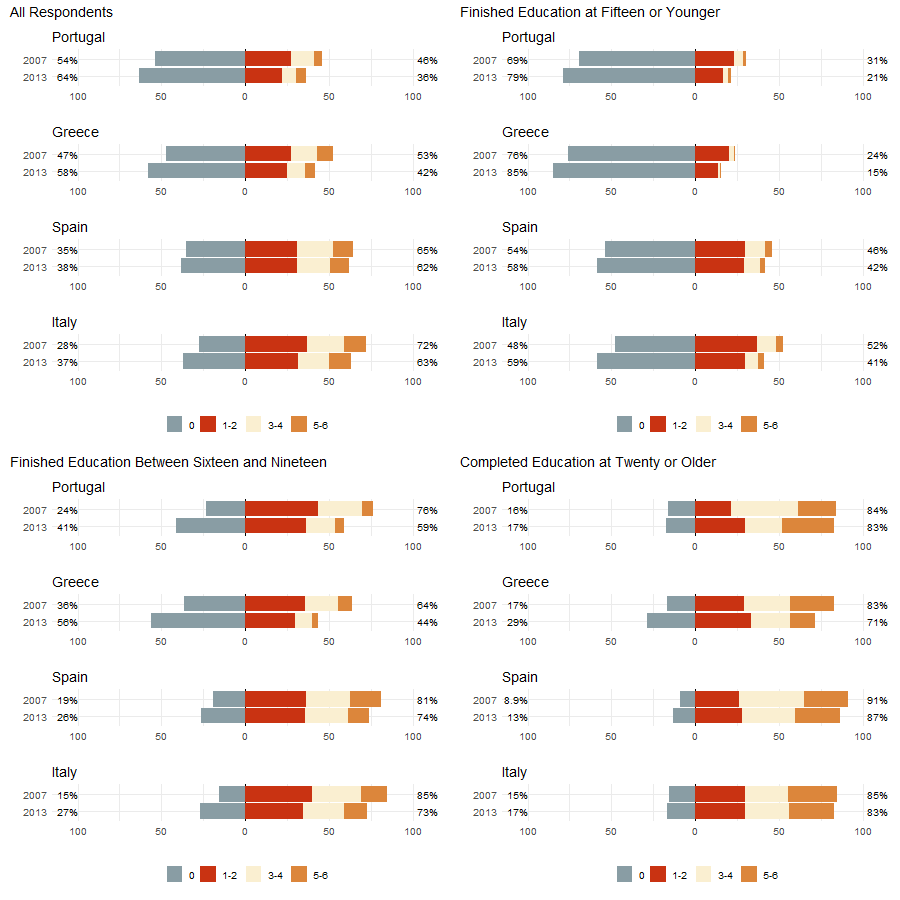
\includegraphics[width=1.0\textwidth]{Plots/cult-cat-by-year-by-country-combo.png}
    \caption{Stacked bar plots of number of cultural activities for four Southern European countries. the top panel (a-b) shows the number of cultural activities per country for 2007 (a) and 2013 (b). The bottom panels (c-j) show the number of cultural activities for each country in each year by the respondent's level of education on the y-axis: Portugal (c-d), Spain (e-f), Italy (g-h) and Greece (i-j).}
    \label{fig: main}
\end{figure}

\section*{References}
\noindent

Bryer, J., \& Speerschneider, K. (2016). Package ‘likert’. Likert: Analysis and Visualization Likert Items, version 1.3, 5, 2016.

Coulangeon, P. (2013). Changing policies, challenging theories and persisting inequalities: Social disparities in cultural participation in France from 1981 to 2008. \textit{Poetics}, 41(2), 177-209.

DiMaggio, P., \& Mukhtar, T. (2004). Arts participation as cultural capital in the United States, 1982–2002: Signs of decline? \textit{Poetics}, 32(2), 169-194.

European Commission (2012). Eurobarometer 67.1 (Feb-Mar 2007). GESIS Data Archive, Cologne. ZA4529 Data file Version 3.0.1. 

European Commission (2016). Eurobarometer 79.2 (Apr-May 2013). GESIS Data Archive, Cologne. ZA5688 Data file Version 6.0.0, 

Heiberger, R., \& Robbins, N. (2014). Design of diverging stacked bar charts for Likert scales and other applications. Journal of Statistical Software, 57, 1-32.

López-Sintas, J., \& Katz-Gerro, T. (2005). From exclusive to inclusive elitists and further: Twenty years of omnivorousness and cultural diversity in arts participation in the USA. \textit{Poetics}, 33(5-6), 299-319.

Ram, K. (2018). wesanderson: a Wes Anderson palette generator. R package version 0.3, 6, 2018.

\end{document}
